\documentclass{article}

\usepackage[T1]{fontenc}
\usepackage[english]{babel}
\usepackage[utf8]{inputenc}

\usepackage{url}
\usepackage{graphicx}
\usepackage{vhistory}
\usepackage{listings}

\def\version {1.0.3}

\title{Gerrit \\ Quick start \\ \small{v\version}}

\author{Paweł Warzecha}
\date{\today}

\begin{document}

\maketitle
\newpage

\tableofcontents
\newpage

\section{Introduction}

Gerrit is a~free, web-based team code collaboration tool. Software developers in a~team can review each other's modifications on their source code using a~Web browser and approve or reject those changes. It integrates closely with Git, a~distributed version control system. Gerrit is a~fork of Rietveld, another code review tool. Both namesakes are of Dutch designer Gerrit Rietveld\cite{Gerrit}.

\section{Using Gerrit}

For this project the GerritHub\cite{GerritHub} is used. It offers free and preconfigured Gerrit server. It has been chosen because it is a~ready to use solution, widely used and integrated with the GitHub. 

Next sections show how to use Gerrit.

\subsection{Registering to GerritHub.io}

To use the GerritHub, the GitHub account is needed. If you don't have a~GitHub account, create it first. Next if You don't have a~GerritHub account click the ``First time Sign In'' button (marked with the red rectangle in the figure~\ref{fig:Register}). Next follow the instructions on the website.

\begin{figure}[!ht]
  \centering
  
\includegraphics[width=.75\textwidth]{img/RegisterToGerritHub}
  \caption{Connecting github.}
  \label{fig:Register}
\end{figure}

\subsection{Cloning repository}

To clone the repository with the project code go to Browse->Projects and in the Filter write the name of the project in which you want to contribute (as shown in figure~\ref{fig:FindProject}). Next click on the project name.

\begin{figure}[!ht]
  \centering
  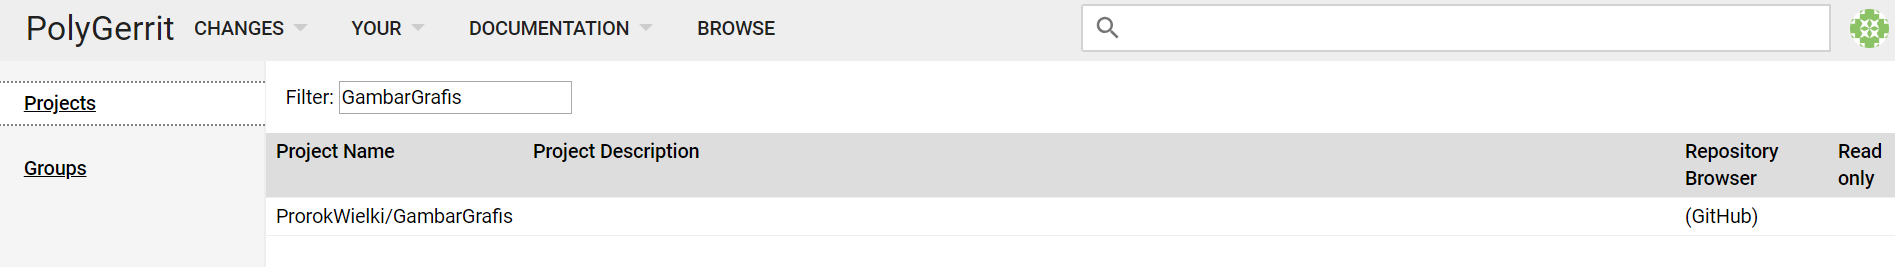
\includegraphics[width=.75\textwidth]{img/FindProject}
  \caption{Finding a~project.}
  \label{fig:FindProject}
\end{figure}

On the site you can see the command which is needed to clone the repository (marked in figure~\ref{fig:Clone})

\begin{figure}[!ht]
  \centering
  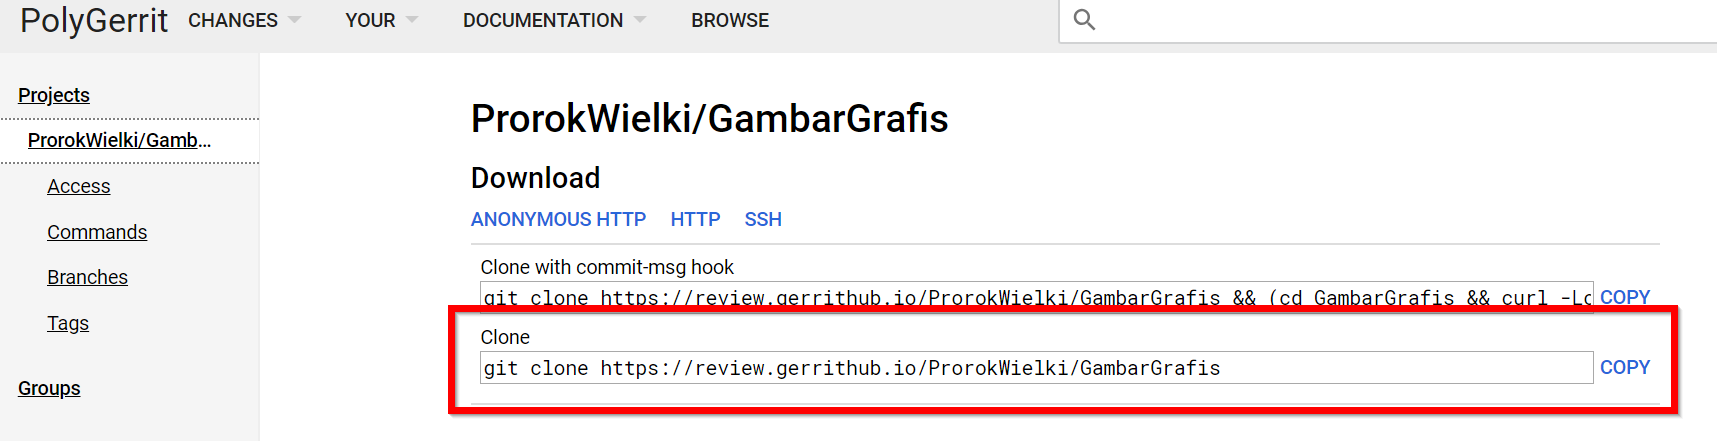
\includegraphics[width=.75\textwidth]{img/Clone}
  \caption{Clone command.}
  \label{fig:Clone}
\end{figure}

\subsection{Pushing changes}

If you want to push your changes to review, just use the git command, but change the branch name in the command to \textit{HEAD:refs/for/<branch\_name>}. For example, if you want to push the changes to a~master branch use: 

\begin{lstlisting}
git push origin HEAD:refs/for/master
\end{lstlisting}

\subsubsection{Adding reviewer}

There are two ways to add reviewer(s) to your change. First, assign the reviewer at the push. In this case use \textit{\%r=<email\_address>} at the end of the push command. The command may look like:

\begin{lstlisting}
git push origin HEAD:refs/for/master%r=ProrokWielki@o2.pl
\end{lstlisting}

The second way is to set the reviewer on the web site. In this case from \textit{YOUR->Changes} select the change to which you want to assign the reviewer. Then on the web page click \textit{ADD REVIEWER}. Put the reviewer email next to the \textit{Reviewers} (as shown in figure~\ref{fig:Reviewer}).

\begin{figure}[!ht]
  \centering
  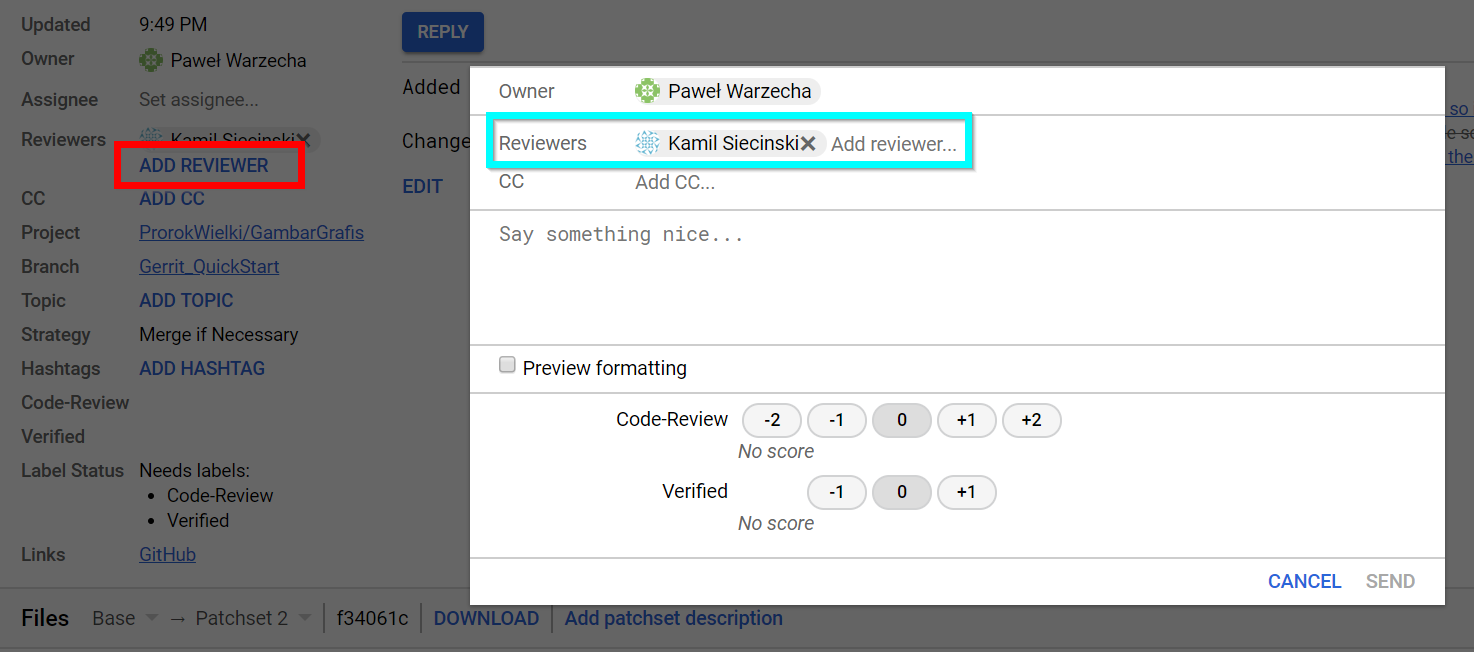
\includegraphics[width=0.75\textwidth]{img/Reviewer}
  \caption{Adding Reviewer.}
  \label{fig:Reviewer}
\end{figure}


\subsubsection{Adding status}

The change can be marked as work in progress (\textit{WIP}). It indicates the change is not yet finished. To set the state to \textit{WIP} you can add the \textit{\%wip} to push command:

\begin{lstlisting}
git push origin HEAD:refs/for/branch_name%wip
\end{lstlisting}

You can also set it from the web page. Go to the change and click \textit{WIP} in the \textit{MORE} menu, as shown in figure~\ref{fig:WIP}.

\begin{figure}[!ht]
  \centering
  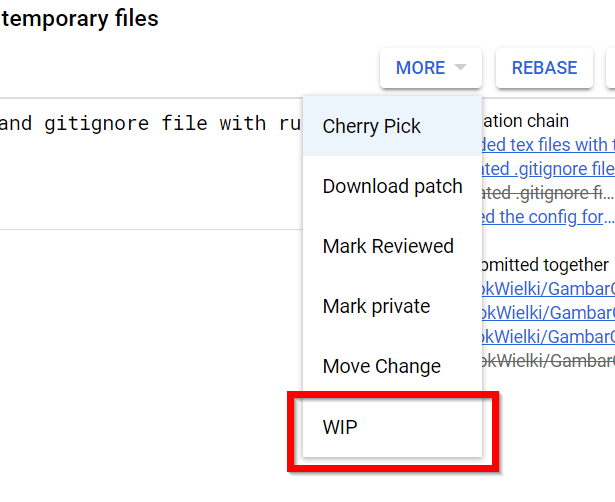
\includegraphics[width=0.5\textwidth]{img/WIP}
  \caption{Setting WIP state.}
  \label{fig:WIP}
\end{figure}


\subsection{Reviewing changes}

If you are asked to review someones change you can see that change in the \textit{Incoming reviews} in the \textit{YOUR->Changes} section.

In the Files Section you can find the files which were pushed with the change. To see the content of a~file, click on its name.

If you want to add comment to a~part of the file, select the text to comment and press \textit{c}. After writing the comment click submit.

After reviewing all files you can mark the change. Click on the \textit{REPLY} button and score the change with points(as shown in figure~\ref{fig:Marking}).

To finish click \textit{SEND}

\begin{figure}[!ht]
  \centering
  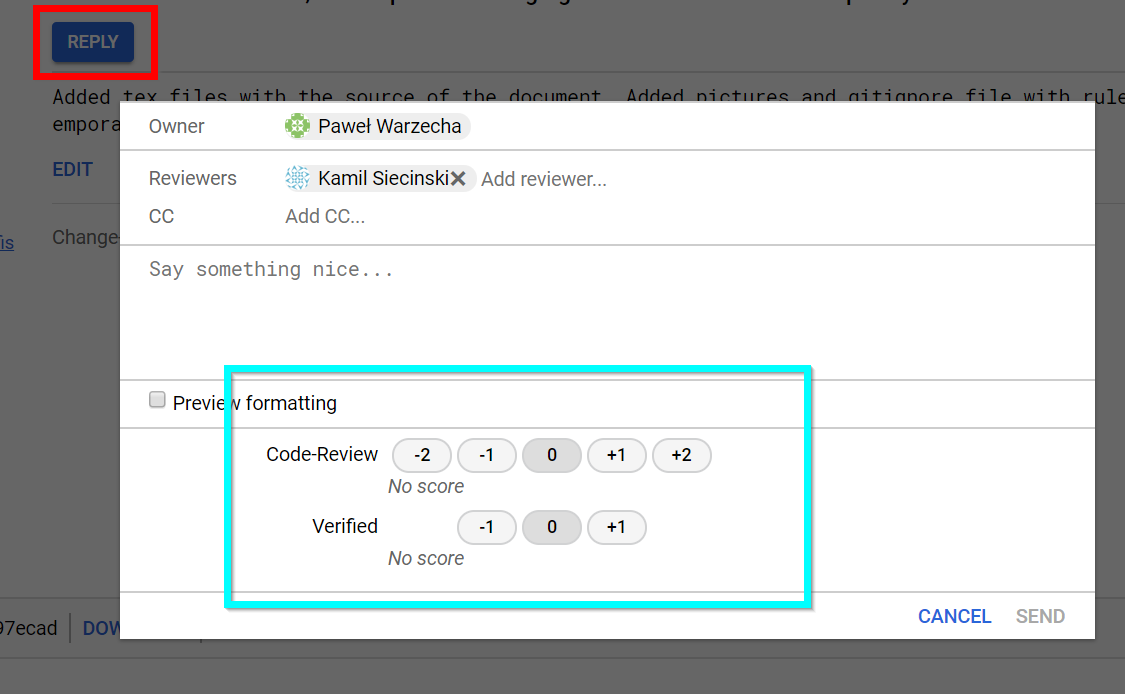
\includegraphics[width=0.75\textwidth]{img/Marking}
  \caption{Marking a~change.}
  \label{fig:Marking}
\end{figure}

\newpage

\subsection{Updating change}

After your change was reviewed, it might happen you need to update something in the change. 

First of all you have to download your change. To do that, on the web page, go to the change. From the \textit{MORE} menu select \textit{Download patch}. From there copy \textit{Checkout} command and run it (shown in figure~\ref{fig:Checkout}).

\begin{figure}[!ht]
  \centering
  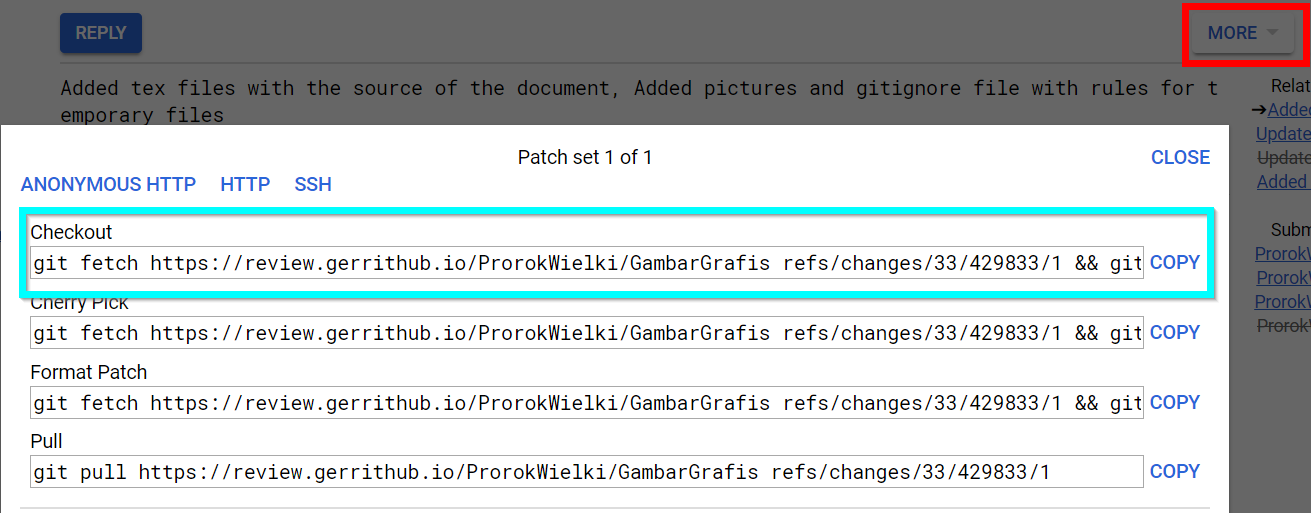
\includegraphics[width=0.75\textwidth]{img/Checkout}
  \caption{Checking out a~change.}
  \label{fig:Checkout}
\end{figure}

Next make necessary changes to the files. After that when committing the change use \textit{--amend} option. And in the comment add the \textit{Change-Id}(as shon in figure~\ref{fig:comment}) associated with the change(can be found on the change web page figure~\ref{fig:changeId}). 

\begin{lstlisting}
git commit --amend
\end{lstlisting}

\begin{figure}[!ht]
  \centering
  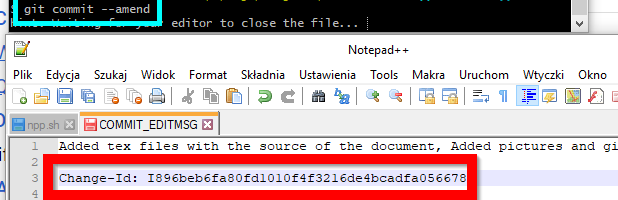
\includegraphics[width=0.5\textwidth]{img/comment}
  \caption{Adding change id.}
  \label{fig:comment}
\end{figure}

\begin{figure}[!ht]
  \centering
  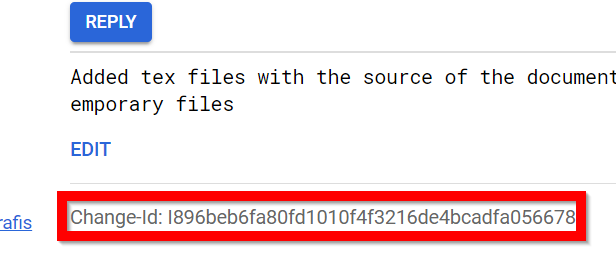
\includegraphics[width=0.5\textwidth]{img/changeID}
  \caption{Change-Id localization.}
  \label{fig:changeId}
\end{figure}

\newpage

After that push the change.


\subsubsection{Changing status to ready}

If your change was in \textit{WIP} status, and after updating the change it is ready to be reviewed add \textit{\%ready} to the push commend.

\begin{lstlisting}
git push origin HEAD:refs/for/branch_name%ready
\end{lstlisting}


\newpage

\begin{thebibliography}{9}

\bibitem{Gerrit} 
\textit{Wikipedia -- Gerrit (software)}.\\ 
\url{https://en.wikipedia.org/wiki/Gerrit_(software)}
 
\bibitem{GerritHub} 
\textit{GerritHub.io}.\\ 
\url{http://gerrithub.io/}

\end{thebibliography}

\newpage

\begin{versionhistory}
  \vhEntry{1.0.0}{18.10.2018}{PW}{Created}
  \vhEntry{1.0.1}{31.10.2018}{PW}{After review -- typos fixed}
  \vhEntry{1.0.2}{1.11.2018}{PW}{After review -- one more typo fixed}
  \vhEntry{1.0.3}{1.11.2018}{PW}{After review -- more typos found and fixed}
\end{versionhistory}

\end{document}
